%-----------------------------------------------------------------
%	SEA SURFACE TEMPERATURE (SST) DATA
%	!TEX root = ./../main.tex
%-----------------------------------------------------------------
\subsection{SST data set}\label{sec:sst}

\subsubsection{Description of the database}\label{ssec:hadisst-intro}
There are several sea surface temperature (SST) databases, with different time-steps (e.g., daily, weekly, monthly, and so on), domains (i.e., global or specific regions), and data resolutions; each used for different analyses of climatological nature~\cite{o:sst-comparison, Rayner2003}.

The Met Office~\cite{o:met-office} Hadley Centre's sea ice and sea surface temperature database, HadISST1~\cite{o:hadisst1}, is a unique combination of monthly globally complete fields of SST and sea ice concentration on a latitude-longitude grid from 1871. In figure~\ref{fig:sst-raster-map} we can see a sample from the data set to illustrate the grid structure. This map has been generated using the function \inline{map_global_sst()} defined in the script~\ref{scr:hadisst_base} in~\cref{app:code}.
\begin{figure}[H]
	\centering
	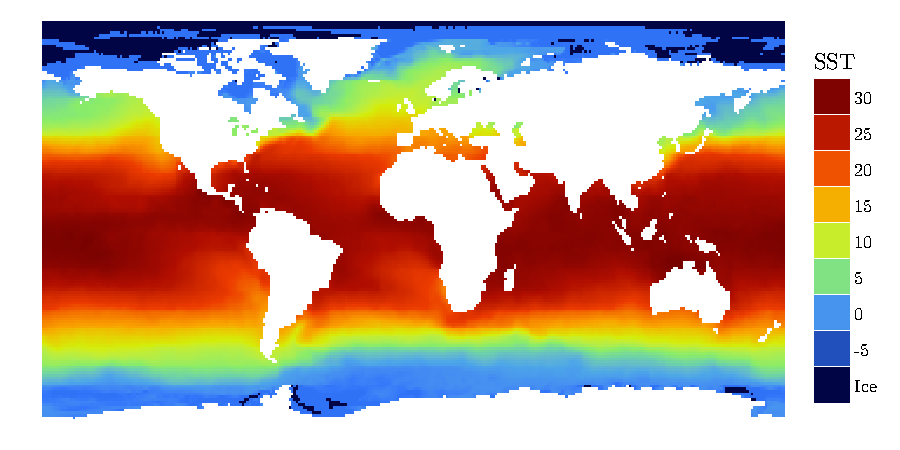
\includegraphics[width=\textwidth]{images/sst-raster-map}
	\caption{Global SST (in \si{\celsius}) map from December 2015}
	\label{fig:sst-raster-map}
\end{figure}

Although there is a revised HadISST.2 database~\cite{o:hadisst2}, we will use the HadISST1 database, as it is the one used in \citeauthor{Corral2010}'s, \citeauthor{Webster2005}'s and several other authors's climate analyses.

The main reason to do so, however, is that HadISST.2 contains more ocean grid boxes and introduces a different method to calculate the monthly temperatures, making it quite incompatible with HadISST1 (as opposed to the revised HURDAT2 database, which is just an improved version of the old database).

%-----------------------------------------------------------------
\subsubsection{Importing and working with raw data}\label{ssec:hadisst-import}
The format of the HadISST1 database is documented at~\cite{o:hadisst1-format}. The particularities of the this database (in ASCII format) are the following:
\begin{itemize}
	\item Temperatures are stored as $\si{\celsius} \times 100$ (all values are integers).
	\item 100\% sea-ice-covered grid-boxes are flagged as \texttt{-1000}.
	\item Land squares are set to \texttt{-32768}.
\end{itemize}

Reading ASCII data, however, can be particularly slow and tedious, as there are several data sets per decade (1870--2003 era) and per year (2004--present era). Thankfully, the HadISST data are also available in netCDF format, which is constructed using raster data instead of just text.

A raster brick consists of a matrix of cells (or pixels) organised into a grid where each cell contains a value representing information, such as temperature in our case. Each matrix can also be comprised of layers (as illustrated in figure~\ref{fig:raster}); in the HadISST1 database, each matrix layer represents a different month.
\begin{figure}[H]
	\centering
	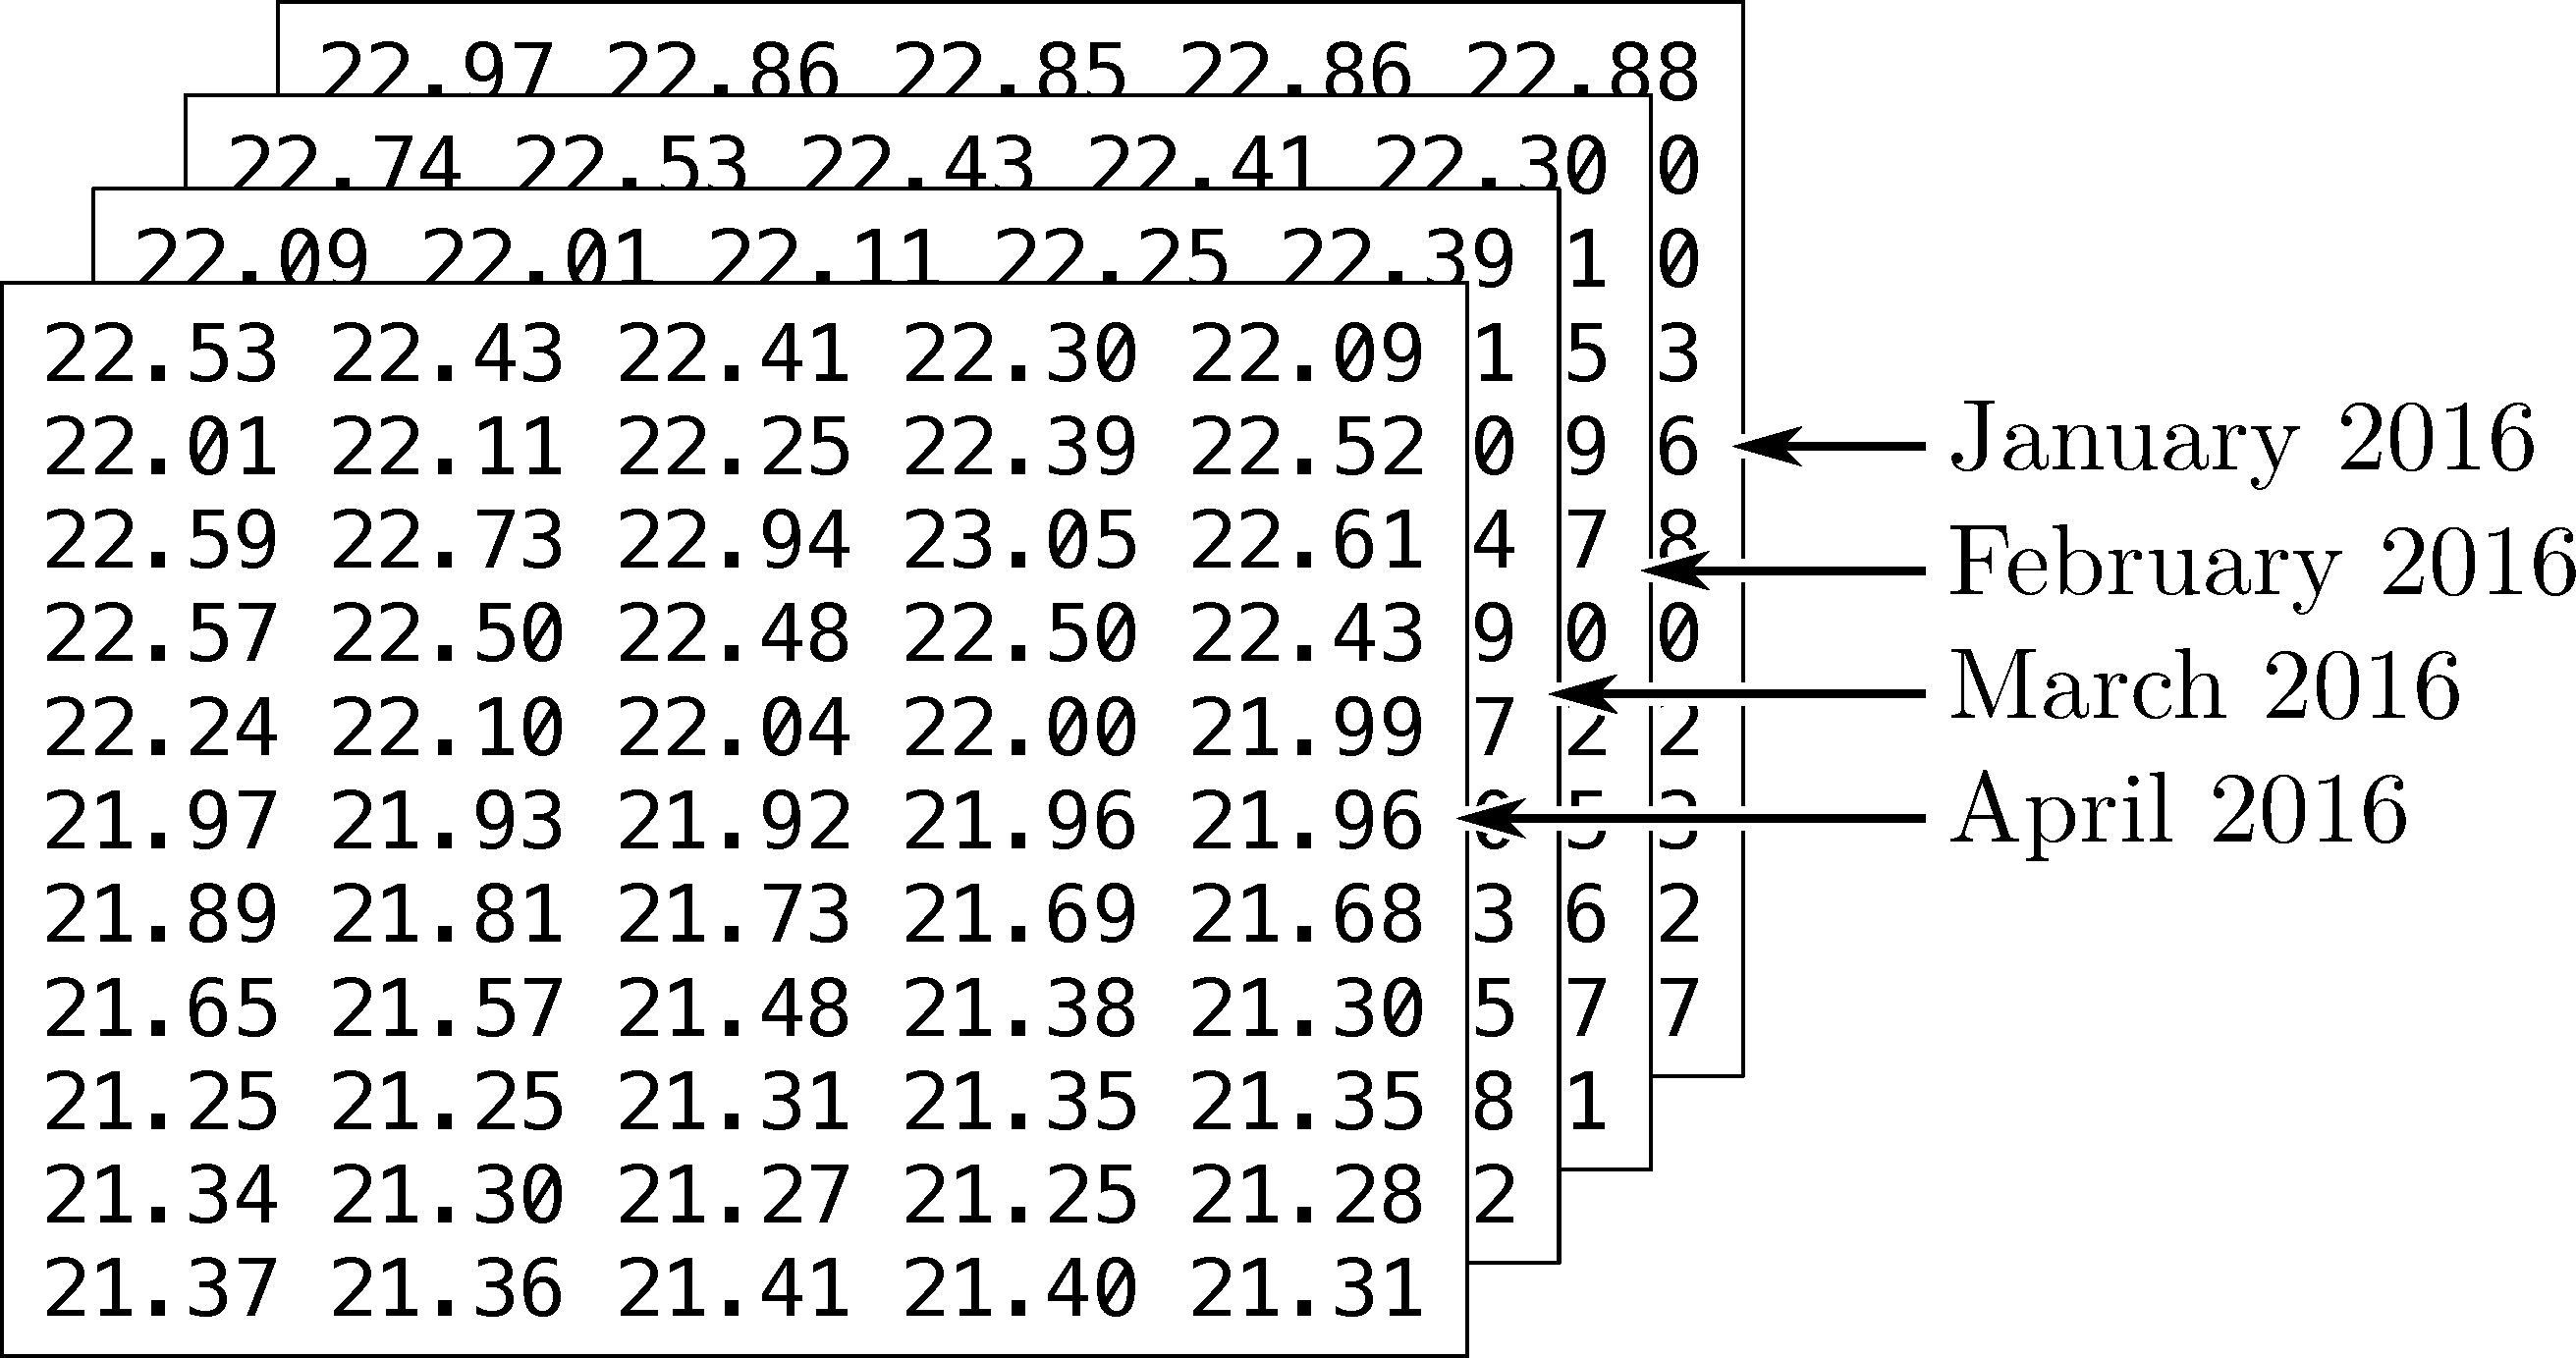
\includegraphics[width=0.7\textwidth]{images/raster}
	\caption{Simple diagram of the internal structure of a raster brick}
	\label{fig:raster}
\end{figure}

The data set used can be downloaded from \url{http://www.metoffice.gov.uk/hadobs/hadisst/data/HadISST_sst.nc.gz}.

\sk
Using the \inline{raster} library in R, we can easily load the HadISST1 raster data:
\begin{lstlisting}[caption=Function to load HasISST data set in netCDF format, label=snp:hadisst-read]
load_hadsst <- function(file = "./HadISST_sst.nc") {
	b <- brick(file)
	NAvalue(b) <- -32768 # Land
	return(b)
}
\end{lstlisting}
Just by doing this we see the clear advantages of using the netCDF format: instead of loading the entire data set, we create a \emph{formal class} raster brick that contains the information about the structure of the \texttt{HadISST\_sst.nc} file, whilst pointing to it. This allows us then to work with the data dynamically (e.g., if we wanted to get the value of an individual SST cell, we would only need the memory necessary to store the actual cell). If we used the ASCII format instead, just reading all \num{114307200} individual SST cells using \inline{data.table} (one of the fastest libraries to read RAW data in R) would have taken a few hours; and this doesn't take into account cleaning and organising the data afterwards.

Note that we do not take into account the 100\% sea-ice-covered grid-boxes (mainly in the Arctic Ocean and small regions of the Antarctic Ocean), as the activity windows are restricted to the tropical regions.

\sk
Now all we need to do is to define a function to read the data from the raster data and get the mean annual (or seasonal to be more precise) SST from a specified region. To do this we crop the raster brick to our desired spatial activity window, and then do the arithmetic mean to get a representative SST value for each year:
\begin{lstlisting}[caption=Function to get mean SSTs data frame from a specific spatial and temporal activity window, label=snp:hadisst-mean-ssts]
get_mean_ssts <- function(x = hadsst.raster, years, range = 6:10,
													coords = c("180W", "180E", "90S", "90N")){
	coords <- morph_coords(coords)
	area <- extent(as.numeric(coords))
	nms <- names(x)
	x <- crop(x, area)

	months <- c("01", "02", "03", "04", "05", "06", "07", "08", "09", "10", "11", "12")
	xMeans <- vector(length = length(years), mode = 'list')
	for (ix in 1:length(years)){
		xMeans[[ix]] <- mean(x[[c(sapply(range,function(x) grep(paste0(years[ix],'.',months[x]),nms)))]], na.rm = T)
	}
	mean.brick <- do.call(brick,xMeans)
	mean.brick <- lapply(1:nlayers(mean.brick),function(ix) mean(as.matrix(mean.brick[[ix]]), na.rm = T))

	mean.df <- unlist(mean.brick)
	mean.df <- data.frame(sst = mean.df)
	mean.df <- classify_ssts(mean.df, years)
	return(mean.df)
}
\end{lstlisting}

Notice that in the snippet ~\ref{snp:hadisst-mean-ssts} we have used the function \inline{classify_ssts()} (snippet~\ref{snp:hadisst-norm}). This function calculates the global basin SST, mathematically defined as
\begin{align}
	\ev{\text{SST}} = \sum_{y} \frac{\text{SST}(y)}{Y}
\end{align}
where $\text{SST}(y)$ is the mean SST of the year $y$, and $Y$ is the total number of years studied; as usual, the standard error of this mean, is defined as
\begin{align}\label{eq:sst-sem}
	SE_{\text{SST}} = \frac{1}{\sqrt{Y}} \sqrt{ \frac{1}{Y-1} \sum_{y} \qty{\text{SST}(y) - \ev{\text{SST}}}^{2} }
\end{align}

The function then classifies each year in low-SST and high-SST years depending on whether they are lower or greater than $\ev{\text{SST}}$.

\begin{lstlisting}[caption=Function to normalise the SSTs and classify years in low or high SST, label=snp:hadisst-norm]
classify_ssts <- function(data.df, years){
	mean.sst <- mean(data.df$sst)
	data.df <- data.df %>%
		mutate(year = as.numeric(substring(rownames(data.df), 1)) + years[1] - 1,
					 year = ymd(paste(year, "01", "01", sep = "-")),
					 sst.norm = sst/mean.sst,
					 sst.class = ifelse(sst.norm >= 1, "high", "low"))
	data.df <- data.df[c("year", "sst", "sst.norm", "sst.class")]
	return(data.df)
}
\end{lstlisting}

As we have stated before, using netCDF is incredibly fast: reading the raster data and computing the necessary calculations merely needs a compile time of \SI{2.639}{s} for the North Atlantic Ocean, and \SI{1.003}{s} for the Northeast Pacific Ocean.

\sk
We commented in~\cref{ssec:hurdat-intro} that the hurricane seasons do not always start and end in the same year for some basins. If we wanted to do deal with these basins, we would need to define an alternative \inline{get_mean_ssts()} function that takes two month ranges (\inline{first.range} and \inline{second.range}) for input (instead of just \texttt{range}), and calculate the mean SST accordingly:
\begin{lstlisting}[caption=Loop to calculate the mean SST in seasons not contained in the same year, label=snp:hadisst-mean-ssts-alt, firstnumber=10]
	for (ix in 2:length(years){
		xMeans[[ix-1]] <- mean(x[[c(sapply(first.range,function(x) grep(paste0(years[ix-1],'.',months[x]), nms)), sapply(second.range,function(x) grep(paste0(years[ix],'.',months[x]), nms)))]], na.rm = T)
	}
\end{lstlisting}

%-----------------------------------------------------------------
\subsubsection{Resulting data structure}
In table~\ref{hd:sst-head} we show the structure of the \inline{ssts.natl} data frame to illustrate the variables we used, as well as the data type of the SST data. Naturally, \inline{ssts.epac} has the same data structure.
\begin{table}[H]
	\centering
	\ttfamily
	\begin{tabular}{r r r r}
		\toprule
		\toprule
		year & sst & sst.norm & sst.class \\
		<date> &   <dbl>   &  <dbl> &    <chr> \\
		\midrule
		1966-01-01 & 27.47 & 0.9979934 &  low \\
		1967-01-01 & 27.19 & 0.9879054 &  low \\
		1968-01-01 & 27.34 & 0.9933687 &  low \\
		1969-01-01 & 27.75 & 1.0083072 & high \\
		1970-01-01 & 27.36 & 0.9940200 &  low \\
		1971-01-01 & 27.04 & 0.9825272 &  low \\
		\bottomrule
	\end{tabular}
	\caption{Excerpt of the \inline{ssts.natl} data frame}
	\label{hd:sst-head}
\end{table}

